\chapter{Data-simulation agreement testing for \texorpdfstring{\BDT}{BDT} training features}\label{sec:appendix_continuum_features_datamc}

All 29 observables that passed the requirements of \textbf{Test~1}, introduced in \Cref{sec:continuum_features}, are subsequently tested in a second test.
This test, named \textbf{Test~2}, aims to test the data-simulation agreement of the features, to ensure that the classifier only learns from features that represent Belle II data adequately.

This is shown, for features that passed \textbf{Test~1} (see \Cref{sec:appendix_continuum_features}) in \Cref{fig:continuum_features_datamc_agreement}.
All but three features show good data-simulation agreement, which attests to the high quality of Belle II detector simulation and calibration.

\begin{figure}[htbp!]
    \centering
    \subcaptionbox{\label{fig:Btag_cosTBTO_agreement_tested}}{
        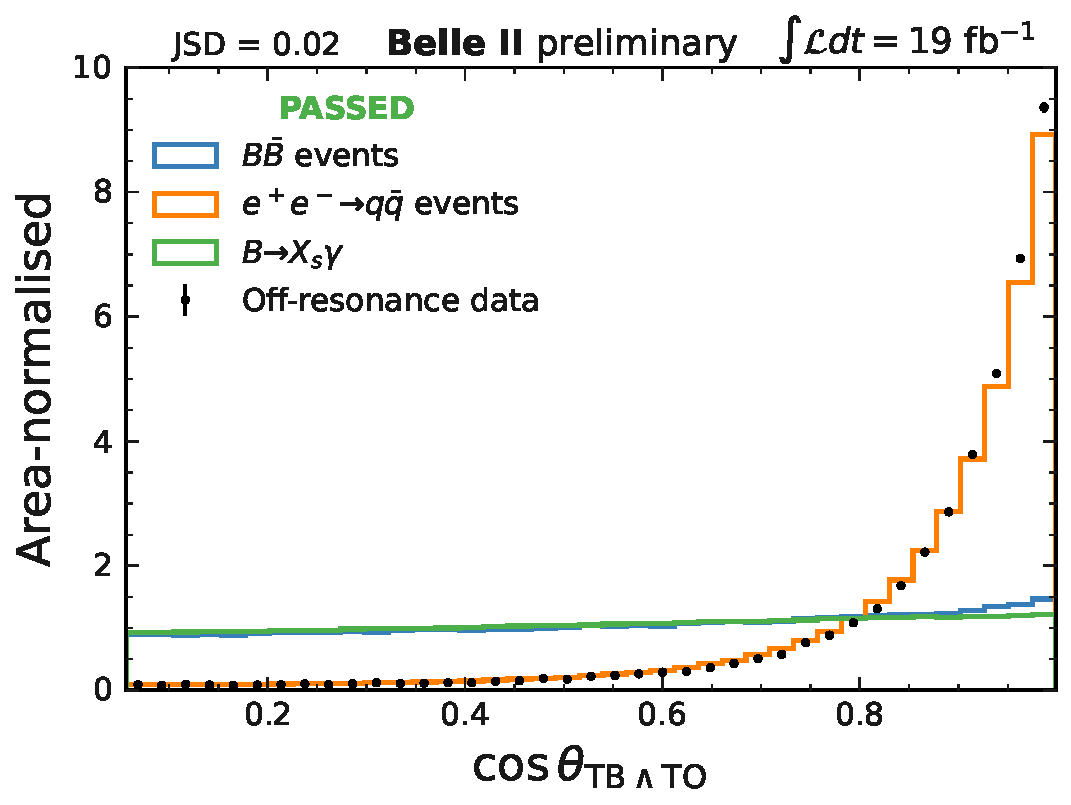
\includegraphics[width=0.3\textwidth]{figures/appendices/continuum_suppression_features/datamc_agreement_tests/Btag_cosTBTO_agreement_tested.pdf}
    }
    \subcaptionbox{\label{fig:Btag_cosTBz_agreement_tested}}{
        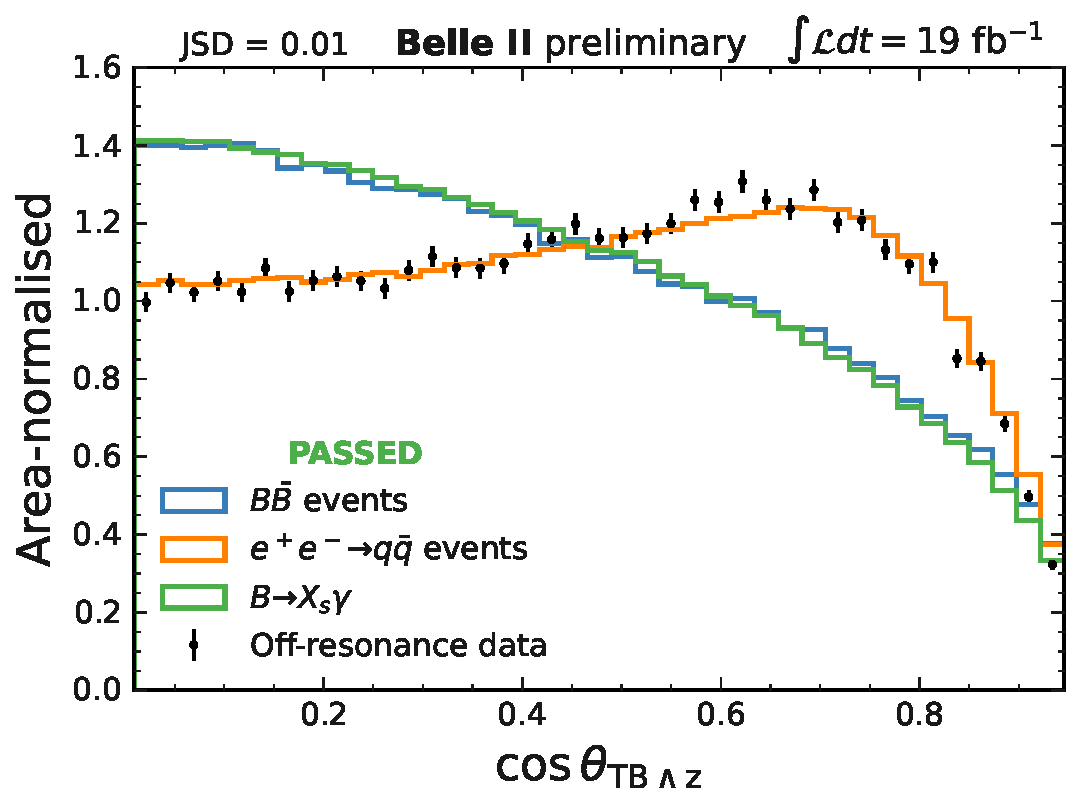
\includegraphics[width=0.3\textwidth]{figures/appendices/continuum_suppression_features/datamc_agreement_tests/Btag_cosTBz_agreement_tested.pdf}
    }
    \subcaptionbox{\label{fig:Btag_thrustBm_agreement_tested}}{
        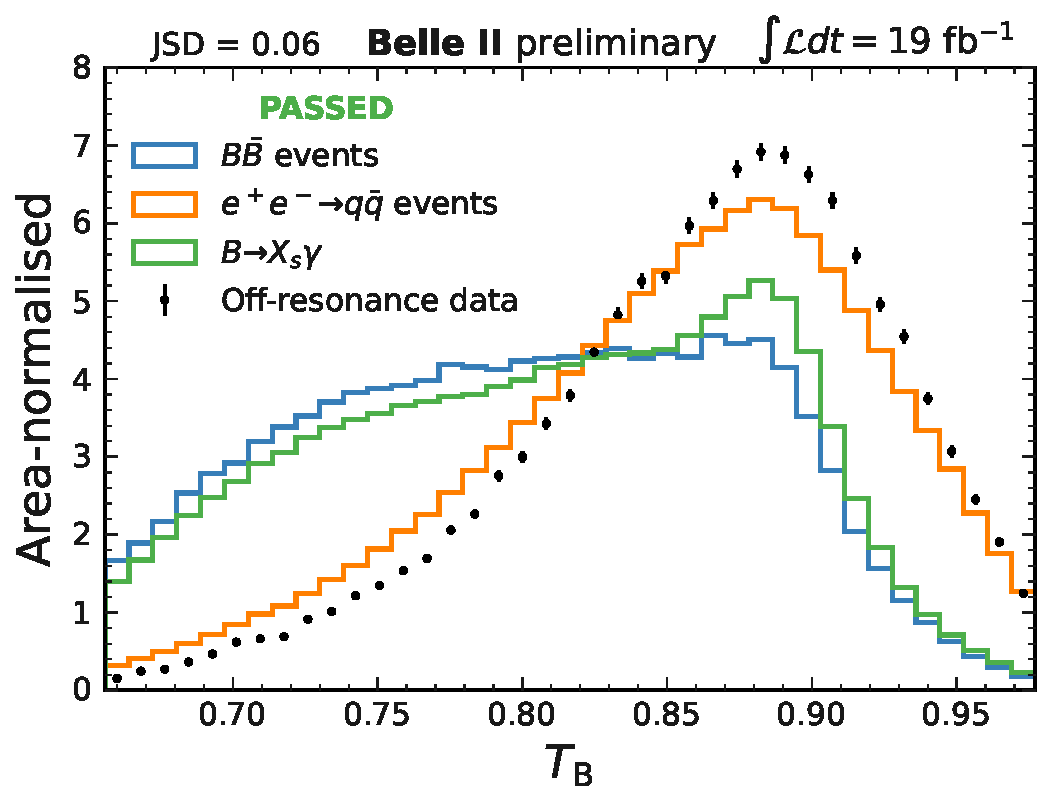
\includegraphics[width=0.3\textwidth]{figures/appendices/continuum_suppression_features/datamc_agreement_tests/Btag_thrustBm_agreement_tested.pdf}
    }
    \subcaptionbox{\label{fig:thrustAxisCosTheta_agreement_tested}}{
        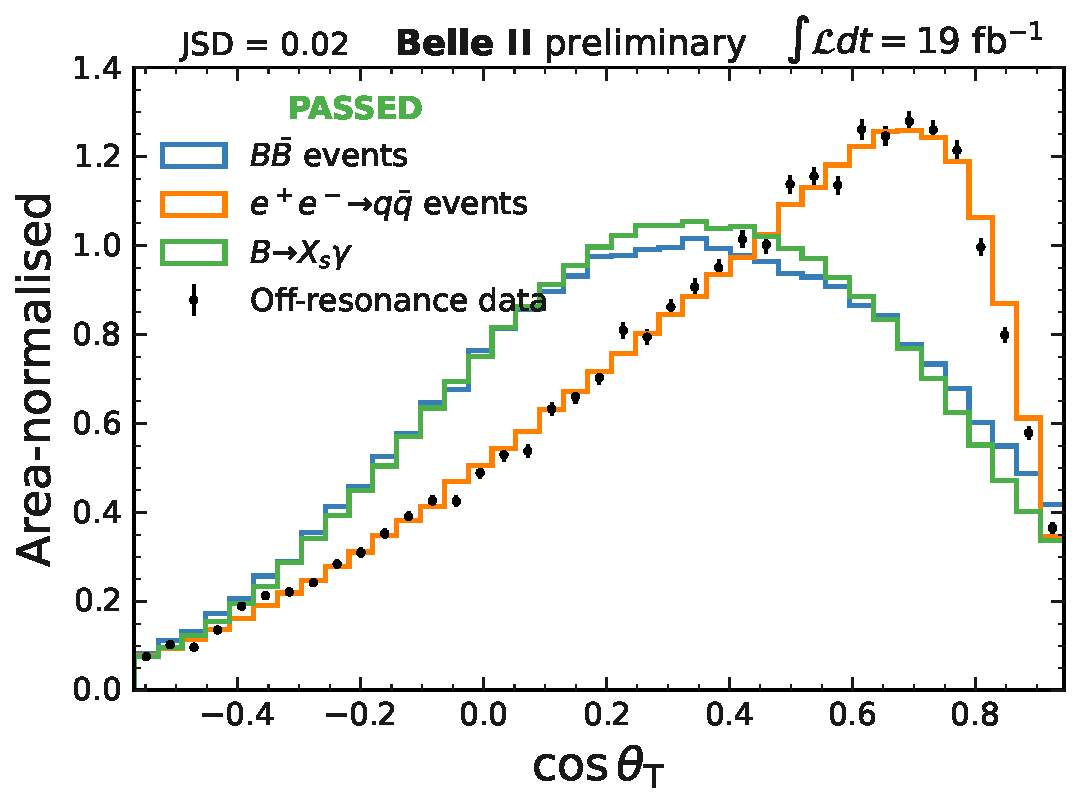
\includegraphics[width=0.3\textwidth]{figures/appendices/continuum_suppression_features/datamc_agreement_tests/thrustAxisCosTheta_agreement_tested.pdf}
    }
    \subcaptionbox{\label{fig:harmonicMomentThrust1_agreement_tested}}{
        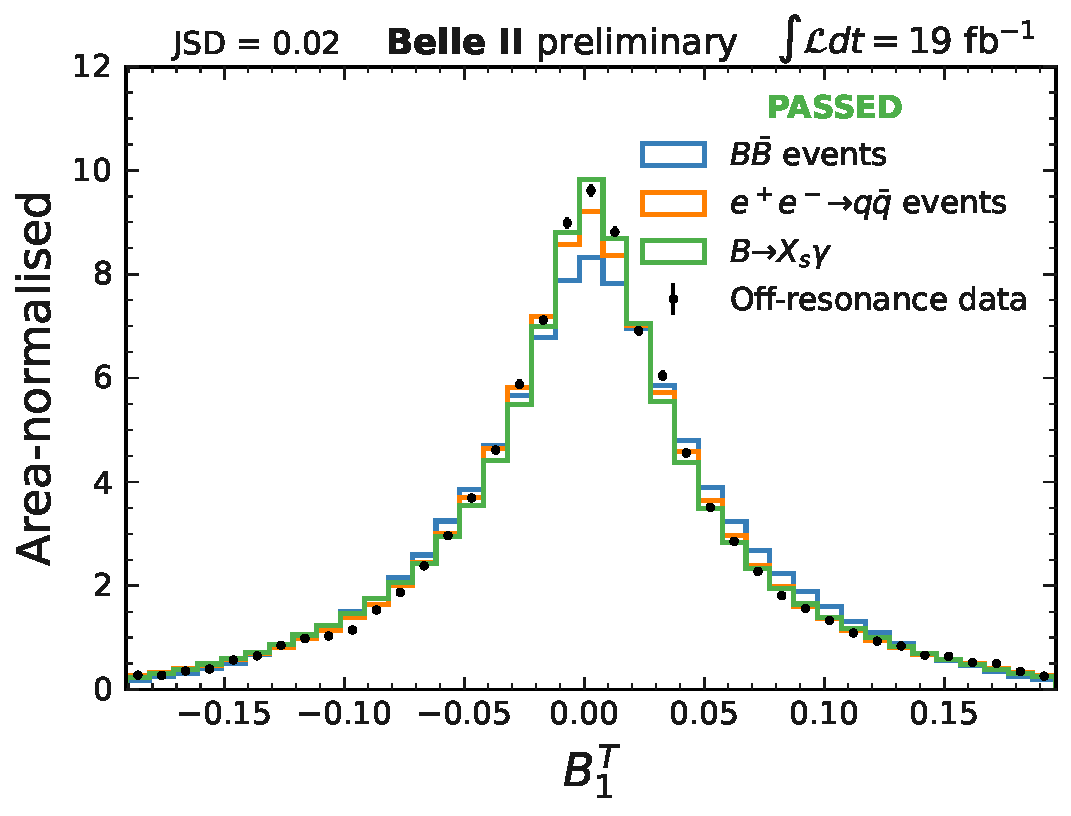
\includegraphics[width=0.3\textwidth]{figures/appendices/continuum_suppression_features/datamc_agreement_tests/harmonicMomentThrust1_agreement_tested.pdf}
    }
    \subcaptionbox{\label{fig:harmonicMomentThrust3_agreement_tested}}{
        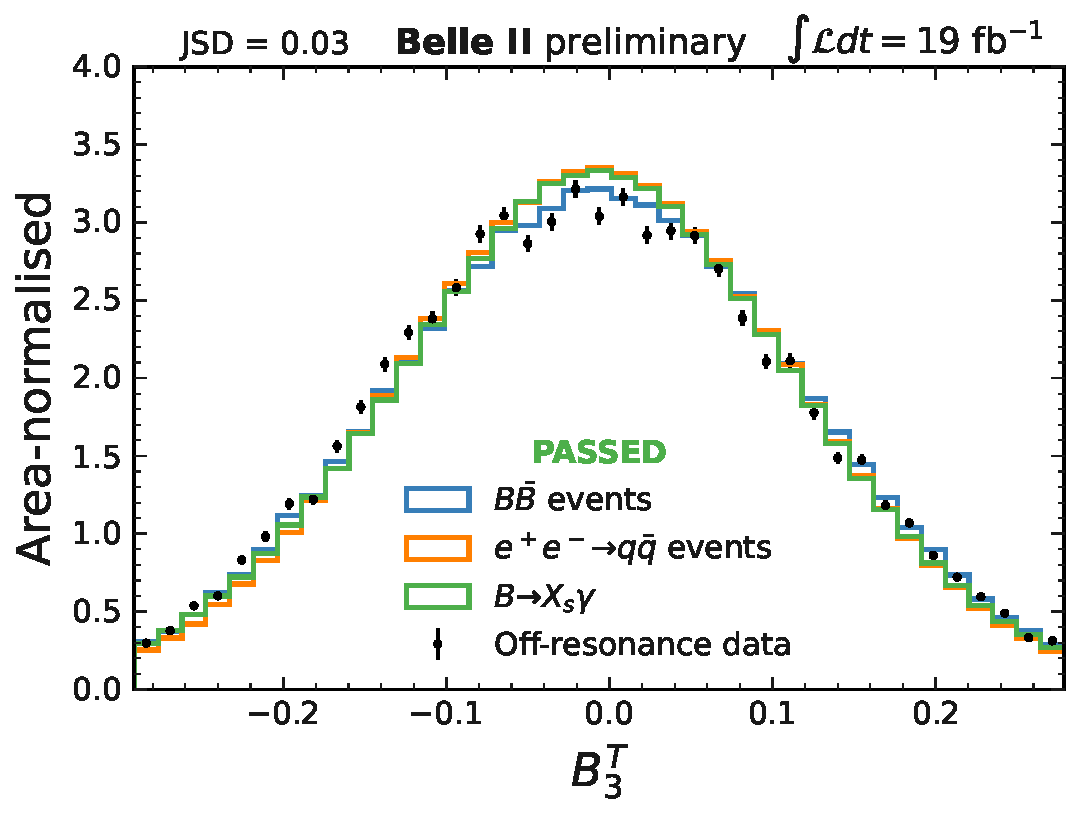
\includegraphics[width=0.3\textwidth]{figures/appendices/continuum_suppression_features/datamc_agreement_tests/harmonicMomentThrust3_agreement_tested.pdf}
    }
\end{figure}
\begin{figure}[htbp!]
    \ContinuedFloat
    \centering
    \subcaptionbox{\label{fig:Btag_CleoCone1_agreement_tested}}{
        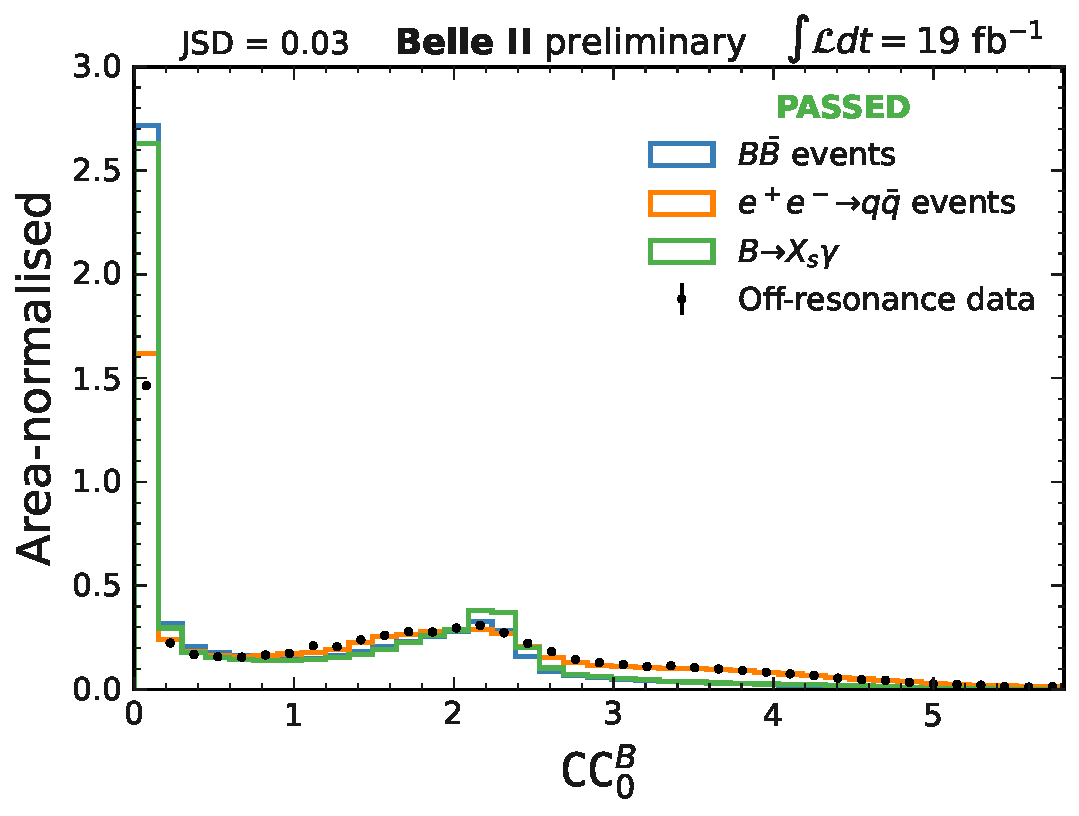
\includegraphics[width=0.3\textwidth]{figures/appendices/continuum_suppression_features/datamc_agreement_tests/Btag_CleoCone1_agreement_tested.pdf}
    }
    \subcaptionbox{\label{fig:Btag_CleoCone2_agreement_tested}}{
        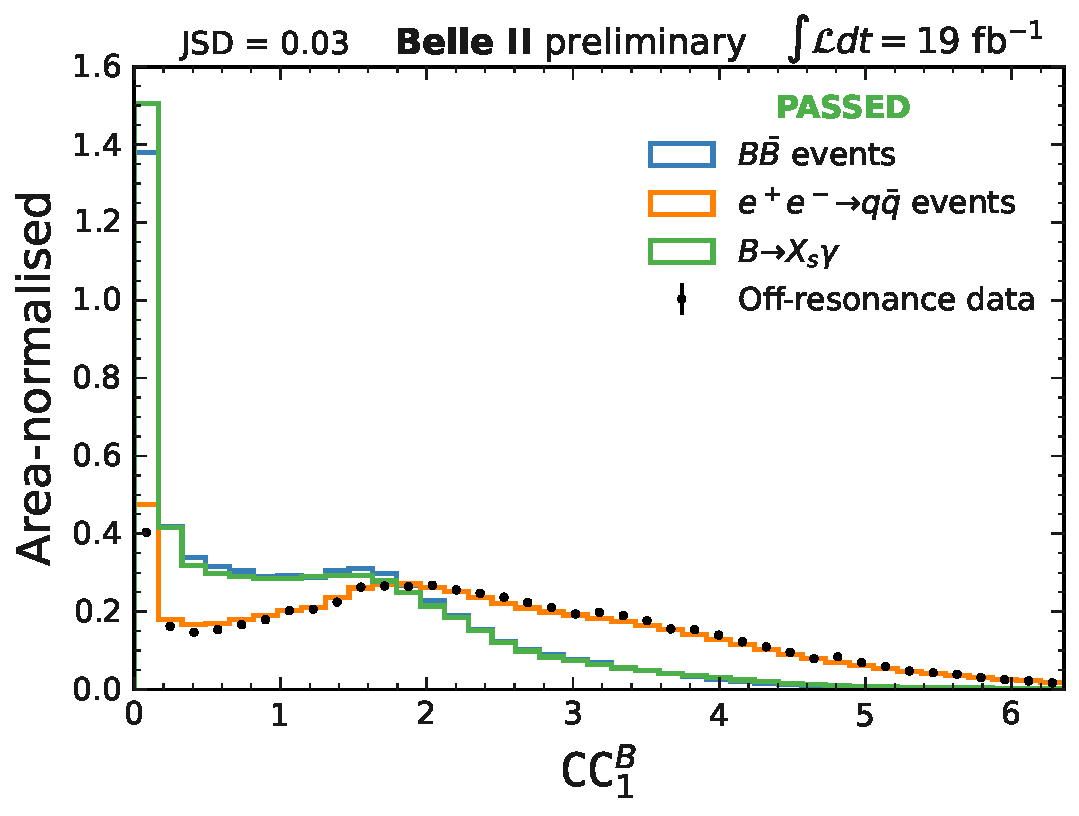
\includegraphics[width=0.3\textwidth]{figures/appendices/continuum_suppression_features/datamc_agreement_tests/Btag_CleoCone2_agreement_tested.pdf}
    }
    \subcaptionbox{\label{fig:Btag_CleoCone3_agreement_tested}}{
        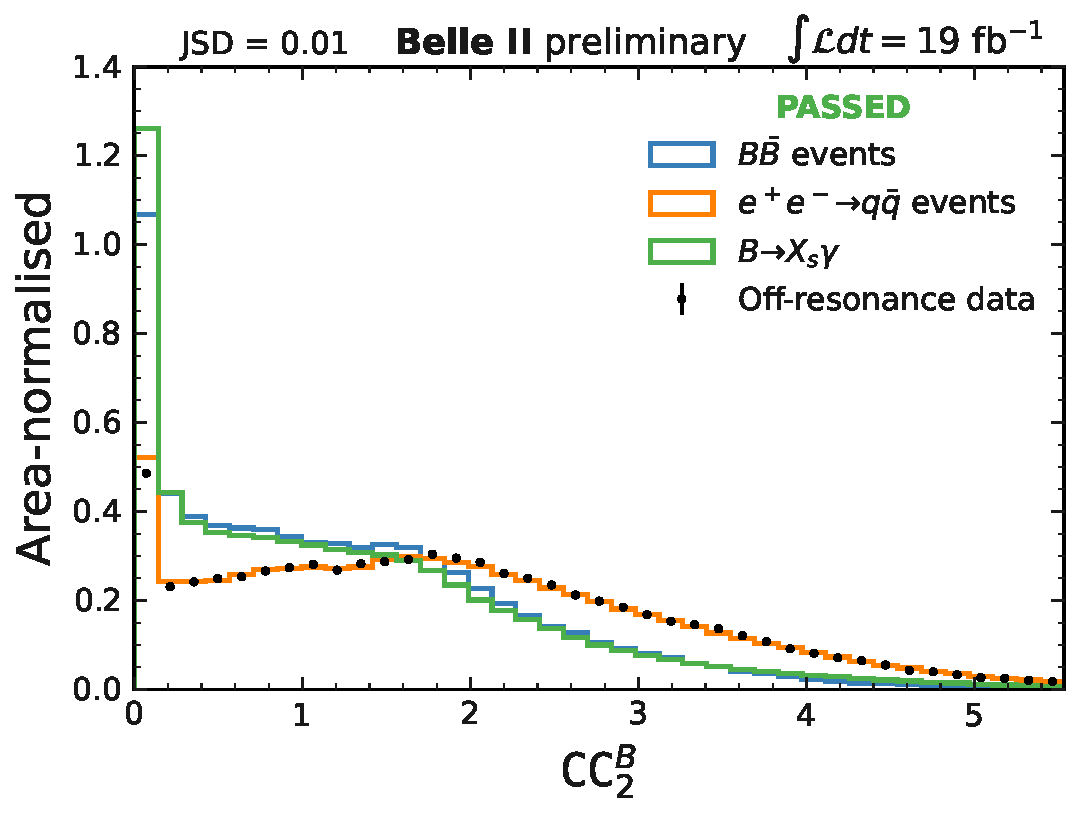
\includegraphics[width=0.3\textwidth]{figures/appendices/continuum_suppression_features/datamc_agreement_tests/Btag_CleoCone3_agreement_tested.pdf}
    }
    \subcaptionbox{\label{fig:Btag_CleoCone4_agreement_tested}}{
        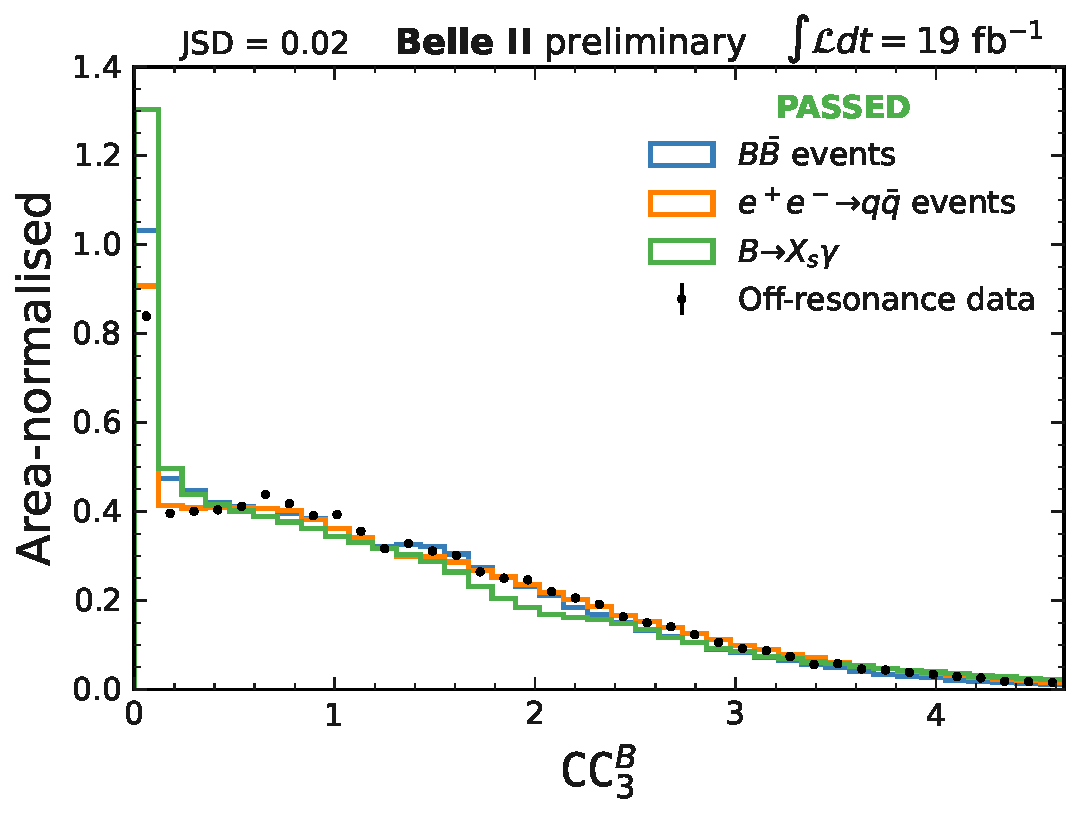
\includegraphics[width=0.3\textwidth]{figures/appendices/continuum_suppression_features/datamc_agreement_tests/Btag_CleoCone4_agreement_tested.pdf}
    }
    \subcaptionbox{\label{fig:cleoConeThrust0_agreement_tested}}{
        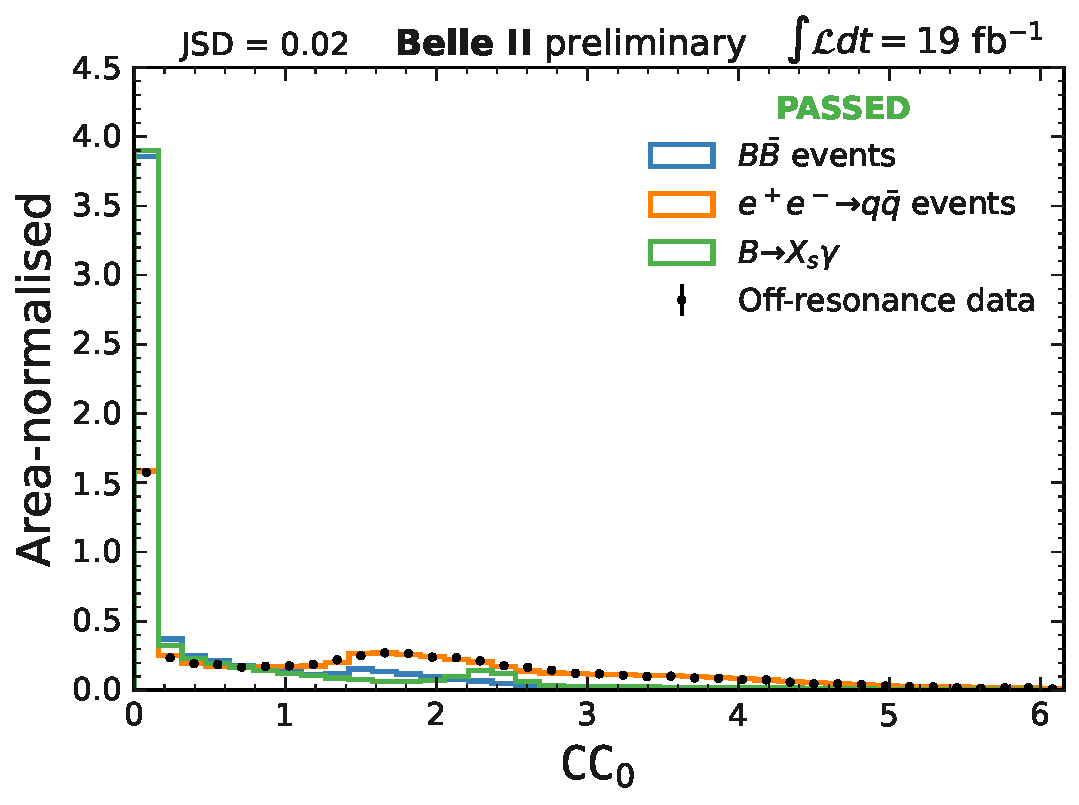
\includegraphics[width=0.3\textwidth]{figures/appendices/continuum_suppression_features/datamc_agreement_tests/cleoConeThrust0_agreement_tested.pdf}
    }
    \subcaptionbox{\label{fig:cleoConeThrust3_agreement_tested}}{
        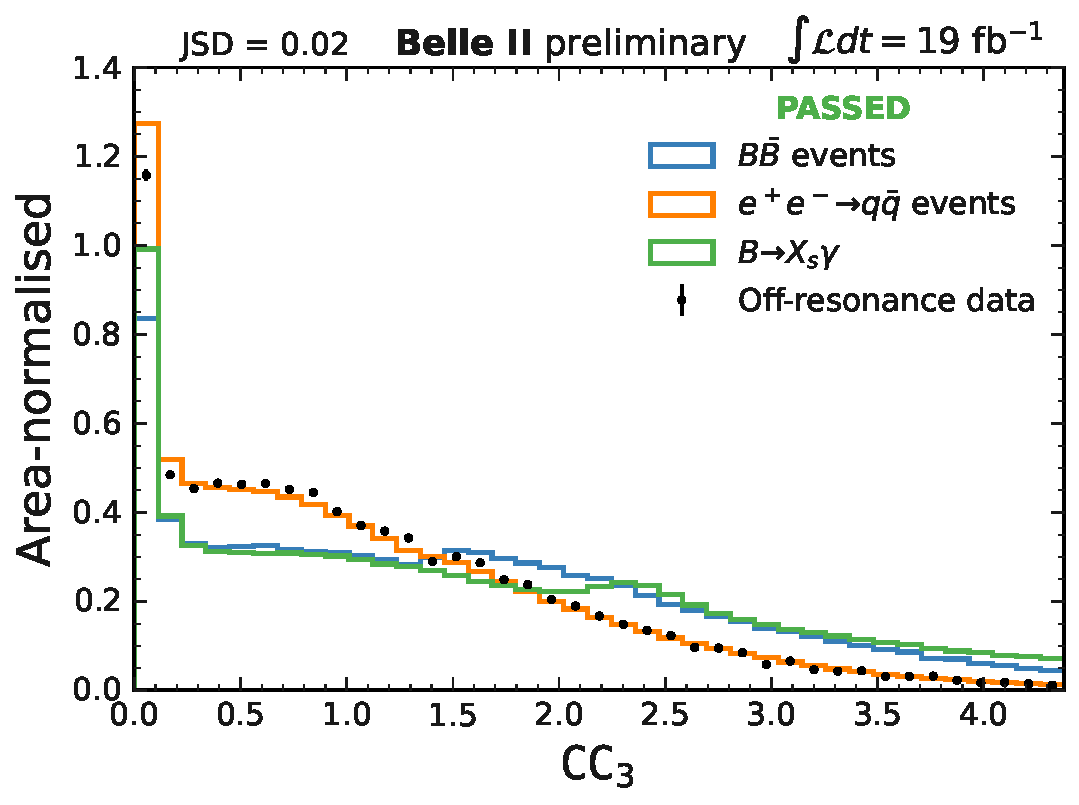
\includegraphics[width=0.3\textwidth]{figures/appendices/continuum_suppression_features/datamc_agreement_tests/cleoConeThrust3_agreement_tested.pdf}
    }
    \subcaptionbox{\label{fig:Btag_KSFW_hso04_agreement_tested}}{
        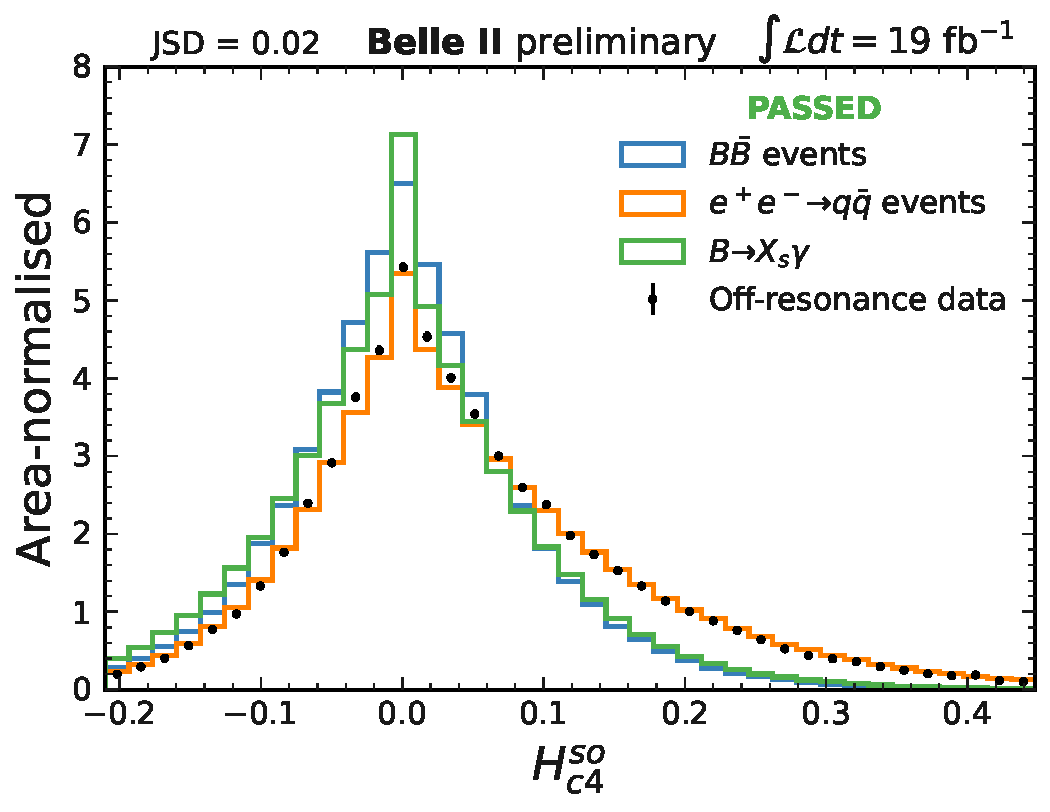
\includegraphics[width=0.3\textwidth]{figures/appendices/continuum_suppression_features/datamc_agreement_tests/Btag_KSFW_hso04_agreement_tested.pdf}
    }
    \subcaptionbox{\label{fig:Btag_KSFW_hso22_agreement_tested}}{
        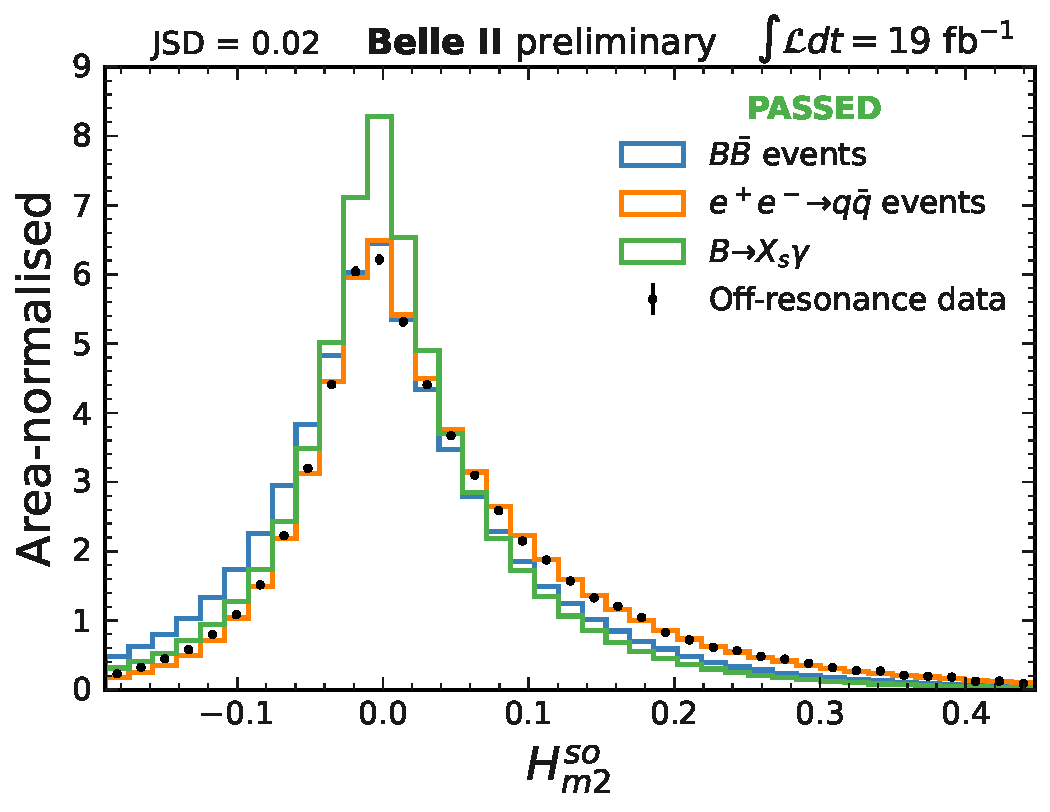
\includegraphics[width=0.3\textwidth]{figures/appendices/continuum_suppression_features/datamc_agreement_tests/Btag_KSFW_hso22_agreement_tested.pdf}
    }
    \subcaptionbox{\label{fig:Btag_KSFW_hso24_agreement_tested}}{
        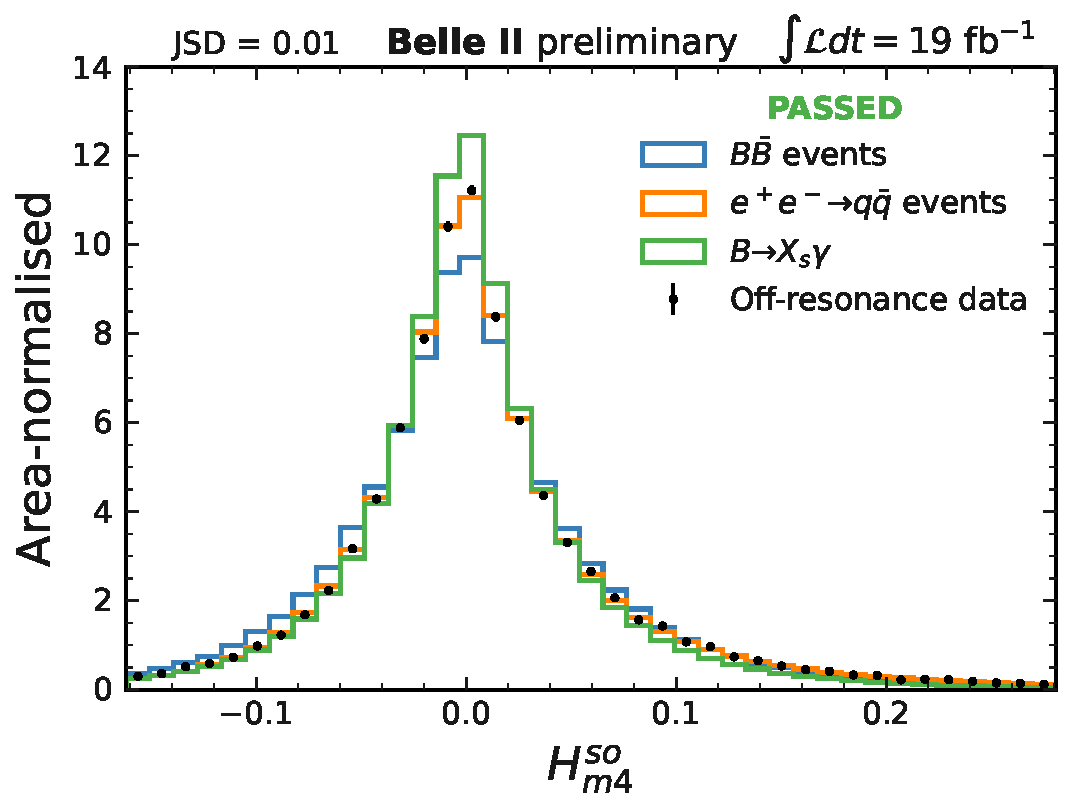
\includegraphics[width=0.3\textwidth]{figures/appendices/continuum_suppression_features/datamc_agreement_tests/Btag_KSFW_hso24_agreement_tested.pdf}
    }
    \subcaptionbox{\label{fig:Btag_KSFW_hoo0_agreement_tested}}{
        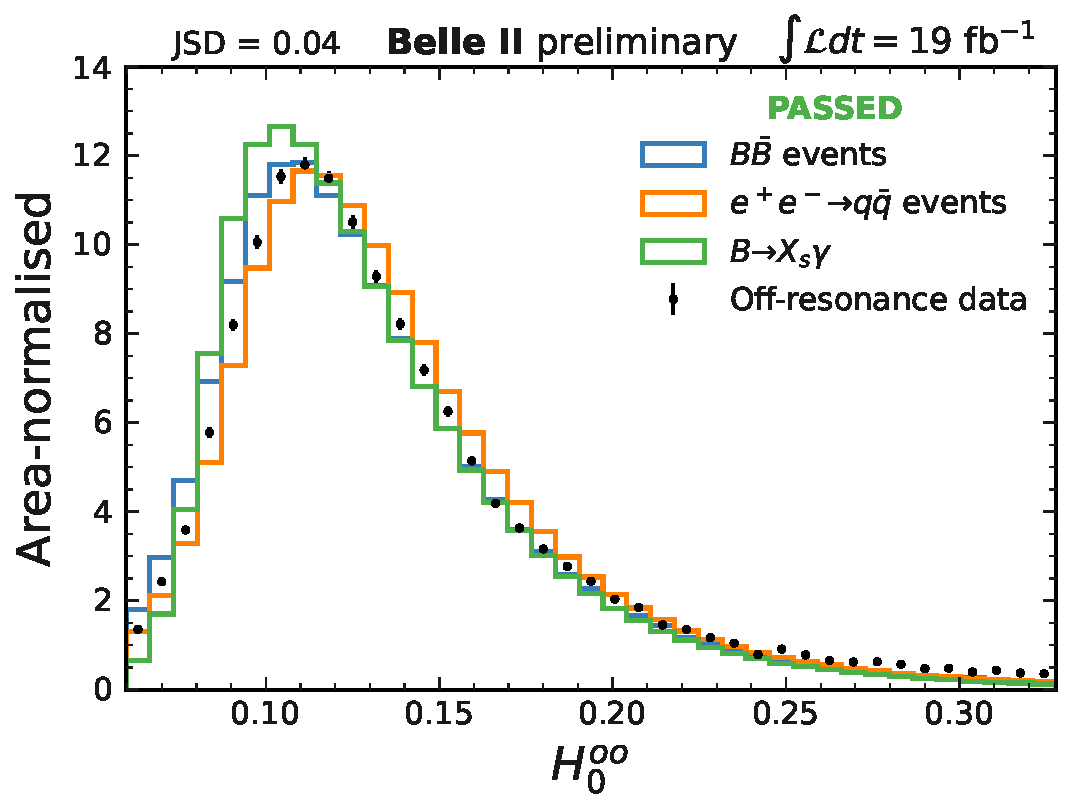
\includegraphics[width=0.3\textwidth]{figures/appendices/continuum_suppression_features/datamc_agreement_tests/Btag_KSFW_hoo0_agreement_tested.pdf}
    }
    % \subcaptionbox{\label{fig:Btag_cosAngleBetweenMomentumAndVertexVectorInXYPlane_agreement_tested}}{
    %     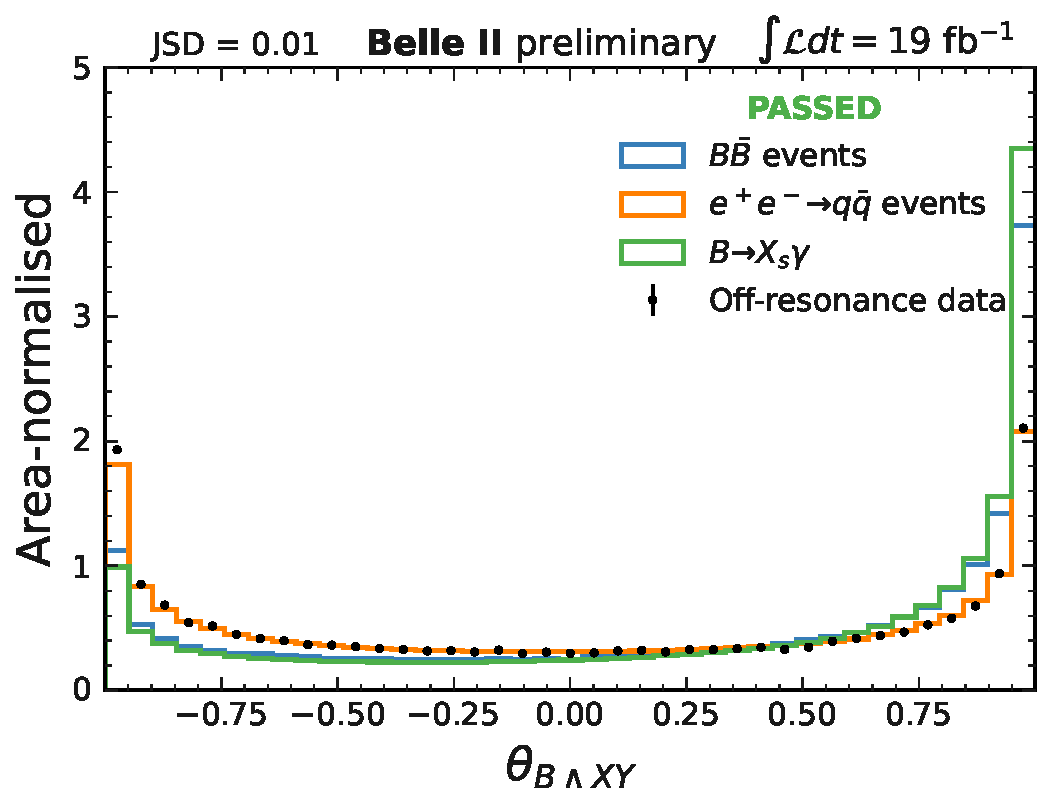
\includegraphics[width=0.3\textwidth]{figures/appendices/continuum_suppression_features/datamc_agreement_tests/Btag_cosAngleBetweenMomentumAndVertexVectorInXYPlane_agreement_tested.pdf}
    % }
    \subcaptionbox{\label{fig:Btag_x_agreement_tested}}{
        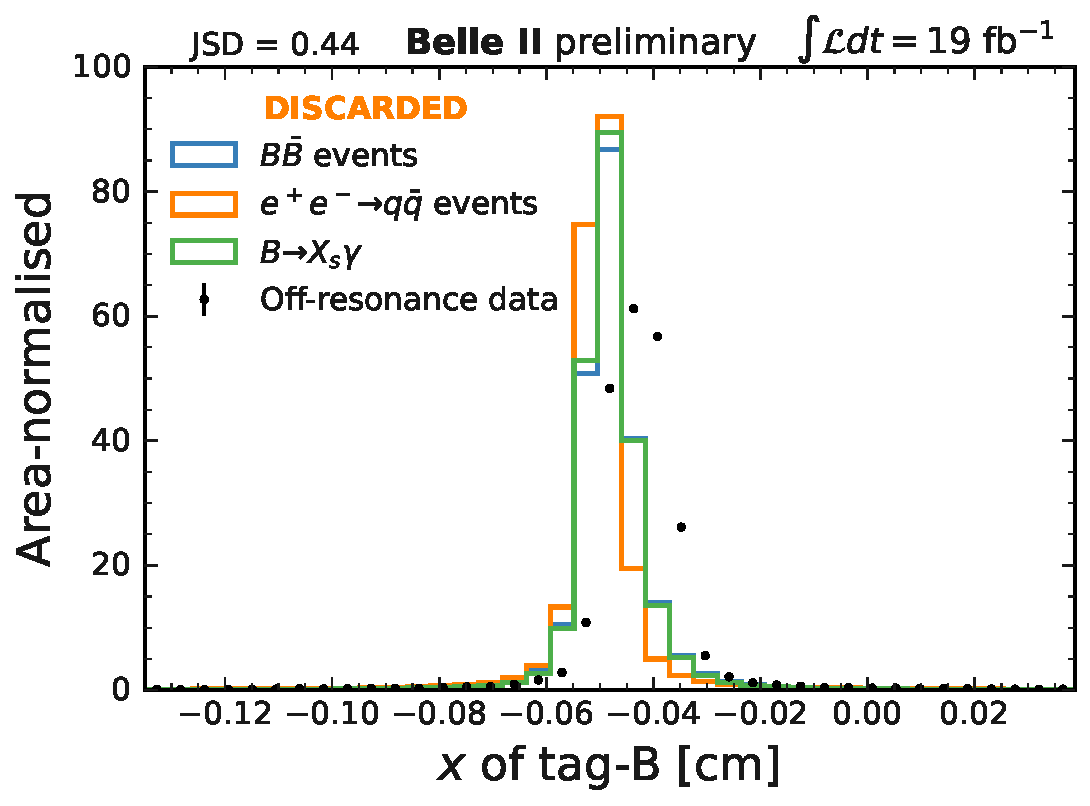
\includegraphics[width=0.3\textwidth]{figures/appendices/continuum_suppression_features/datamc_agreement_tests/Btag_x_agreement_tested.pdf}
    }
        \subcaptionbox{\label{fig:Btag_y_agreement_tested}}{
        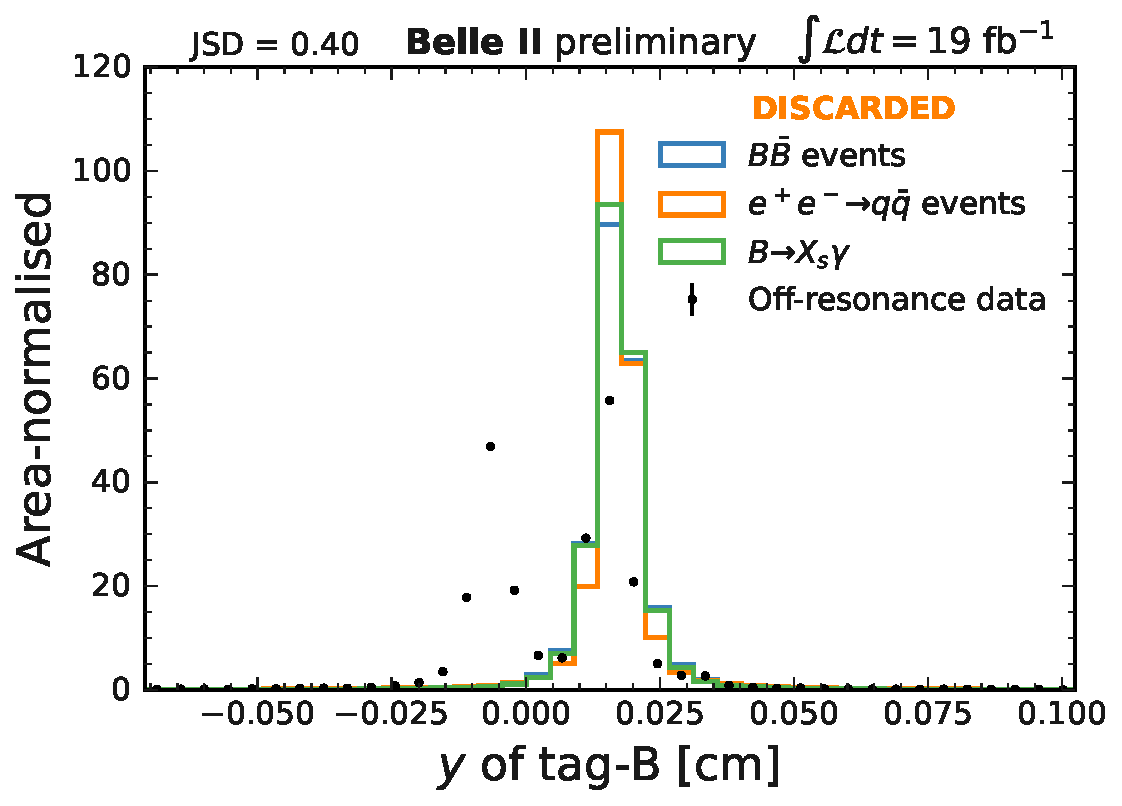
\includegraphics[width=0.3\textwidth]{figures/appendices/continuum_suppression_features/datamc_agreement_tests/Btag_y_agreement_tested.pdf}
    }


\end{figure}
\begin{figure}[htbp!]
    \ContinuedFloat
    \centering
    \subcaptionbox{\label{fig:Btag_z_agreement_tested}}{
        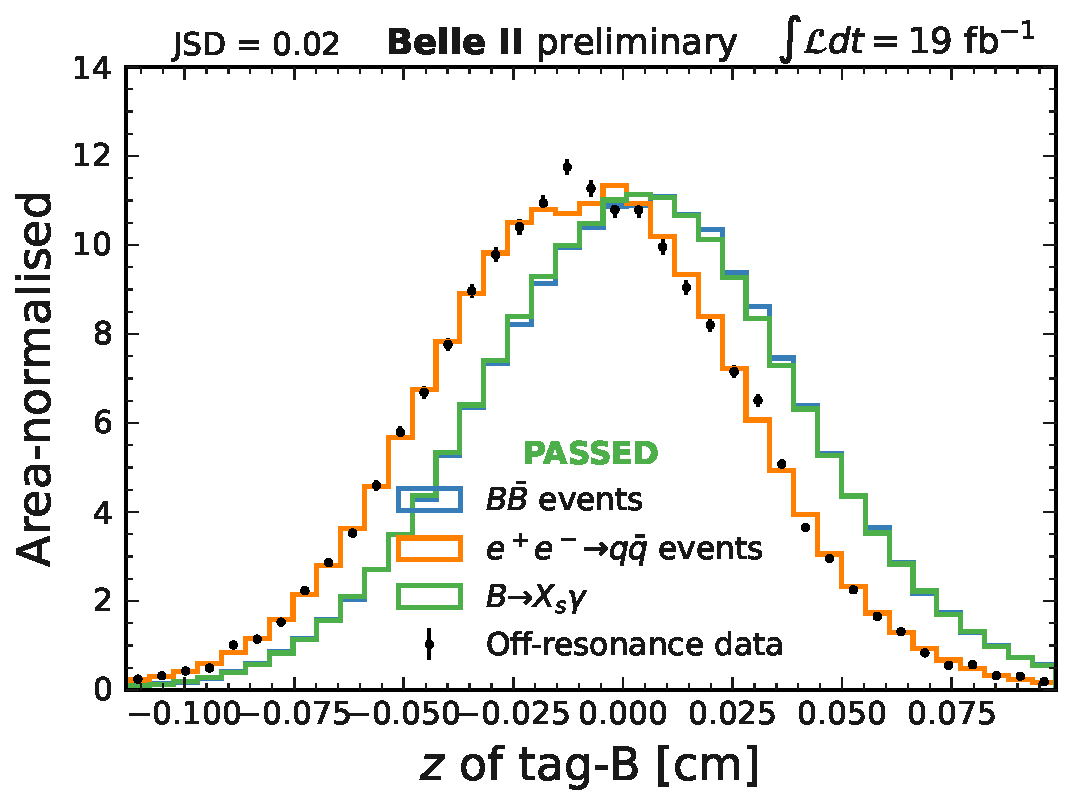
\includegraphics[width=0.3\textwidth]{figures/appendices/continuum_suppression_features/datamc_agreement_tests/Btag_z_agreement_tested.pdf}
    }
    \subcaptionbox{\label{fig:Btag_x_uncertainty_agreement_tested}}{
        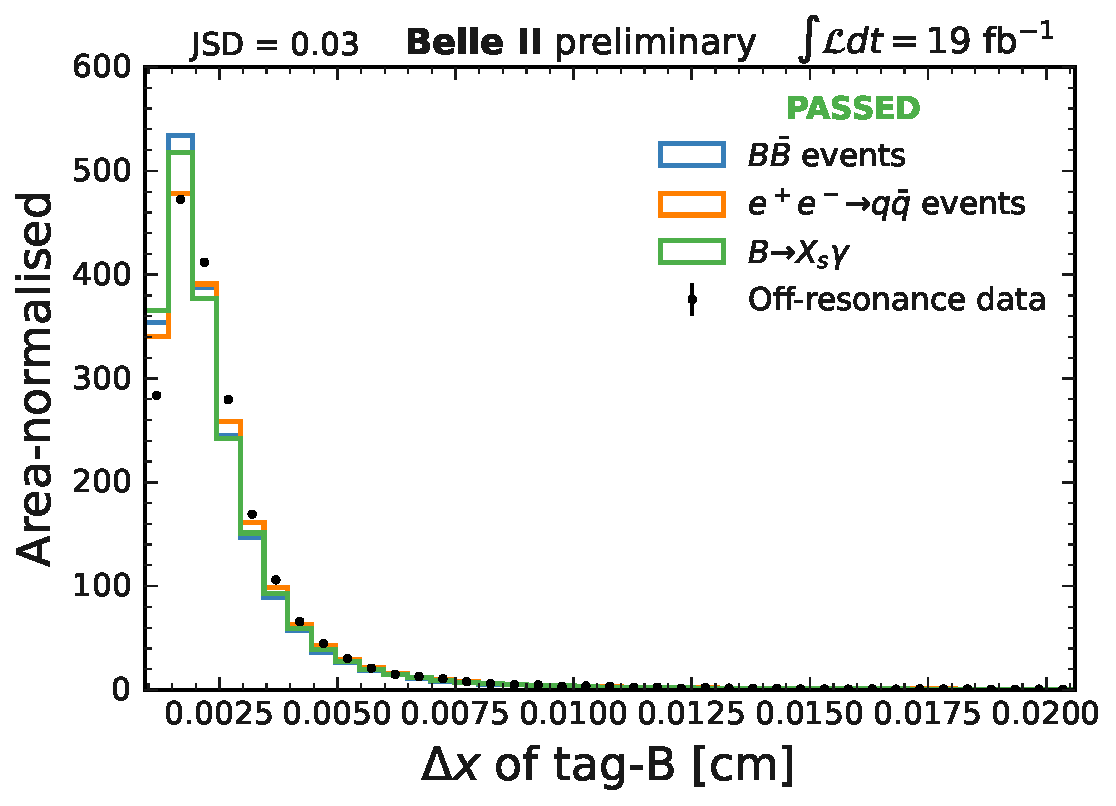
\includegraphics[width=0.3\textwidth]{figures/appendices/continuum_suppression_features/datamc_agreement_tests/Btag_x_uncertainty_agreement_tested.pdf}    
    }
    \subcaptionbox{\label{fig:Btag_y_uncertainty_agreement_tested}}{
        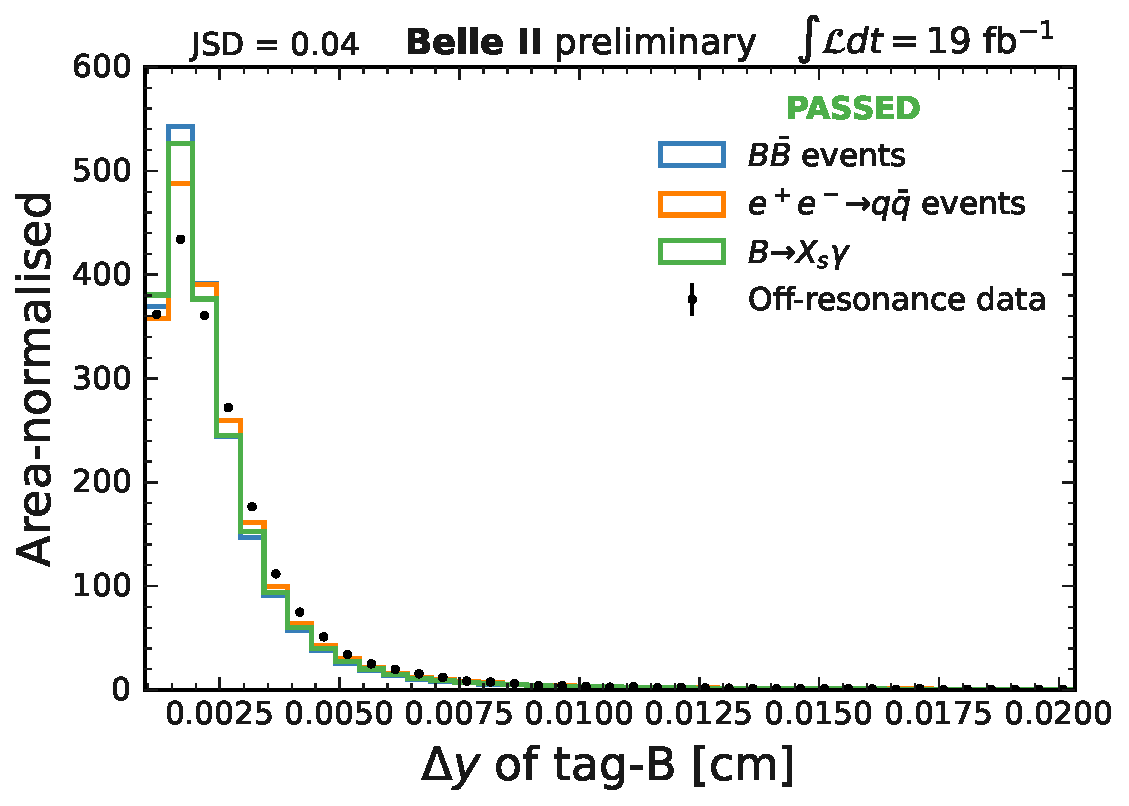
\includegraphics[width=0.3\textwidth]{figures/appendices/continuum_suppression_features/datamc_agreement_tests/Btag_y_uncertainty_agreement_tested.pdf}    
    }
    \subcaptionbox{\label{fig:Btag_z_uncertainty_agreement_tested}}{
        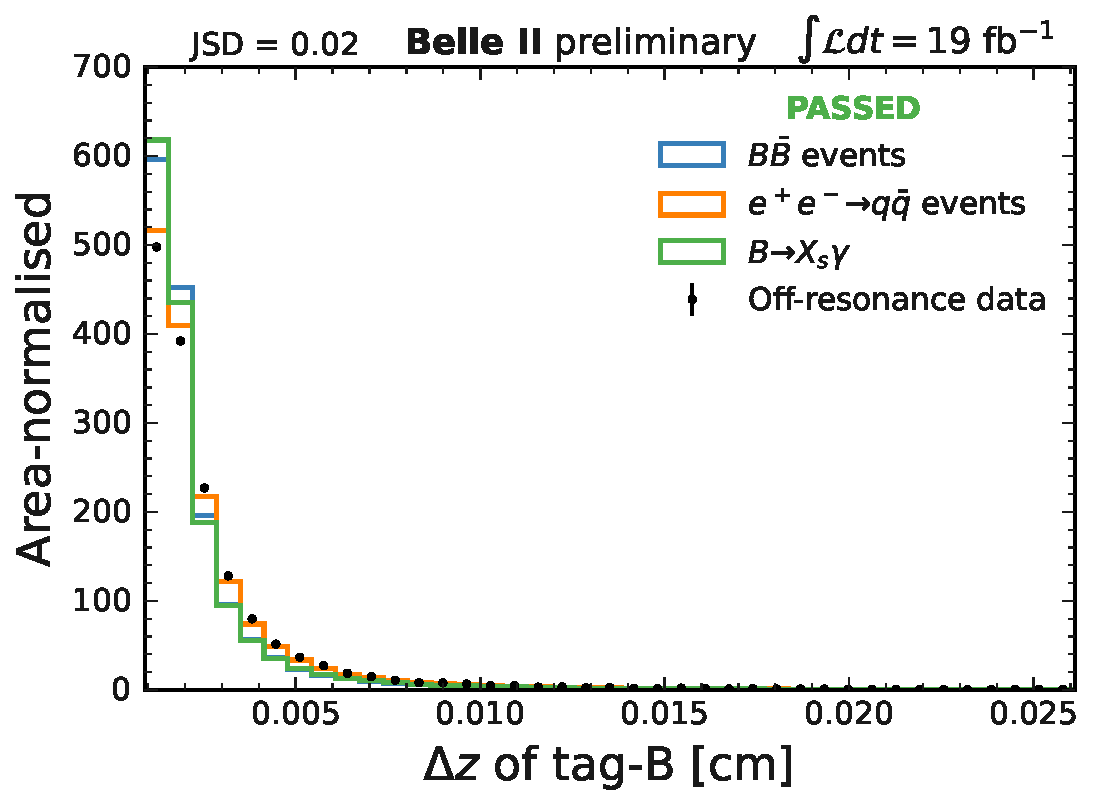
\includegraphics[width=0.3\textwidth]{figures/appendices/continuum_suppression_features/datamc_agreement_tests/Btag_z_uncertainty_agreement_tested.pdf}    
    }
    % \subcaptionbox{\label{fig:Btag_chiProb_agreement_tested}}{
    %     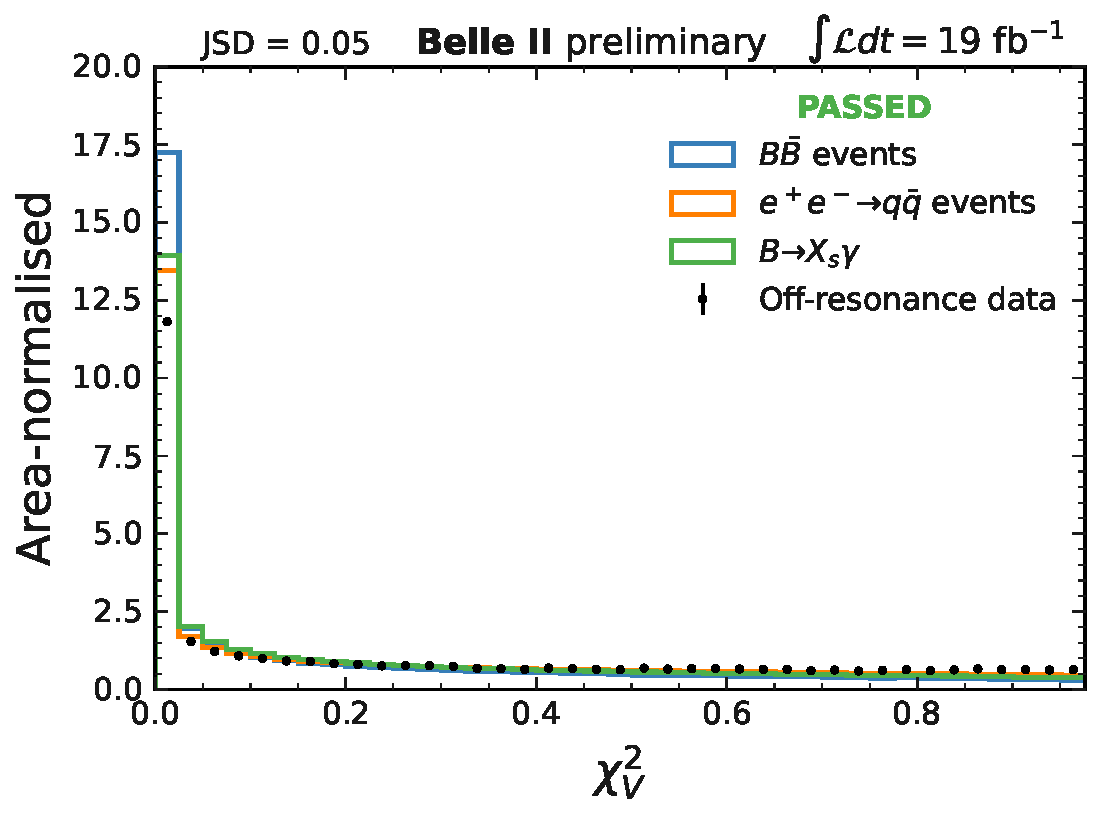
\includegraphics[width=0.3\textwidth]{figures/appendices/continuum_suppression_features/datamc_agreement_tests/Btag_chiProb_agreement_tested.pdf}    
    % }
    \subcaptionbox{\label{fig:Btag_DeltaT_agreement_tested}}{
        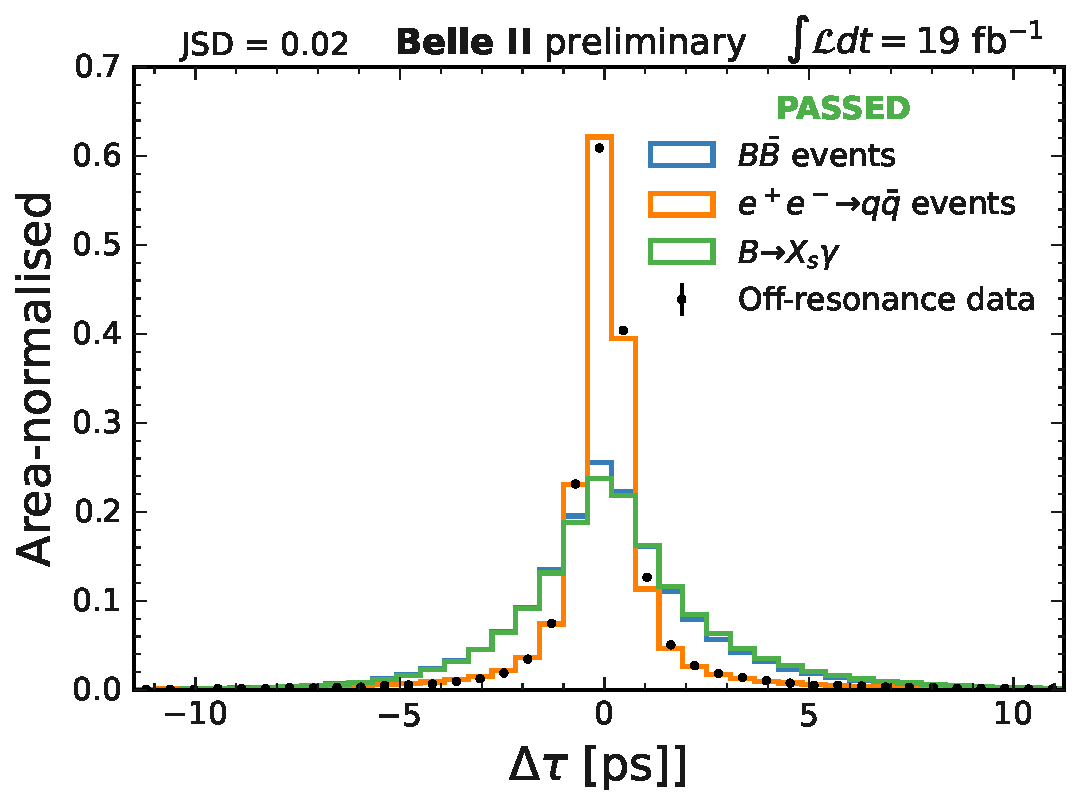
\includegraphics[width=0.3\textwidth]{figures/appendices/continuum_suppression_features/datamc_agreement_tests/Btag_DeltaT_agreement_tested.pdf}    
    }
    \subcaptionbox{\label{fig:Btag_DeltaZ_agreement_tested}}{
        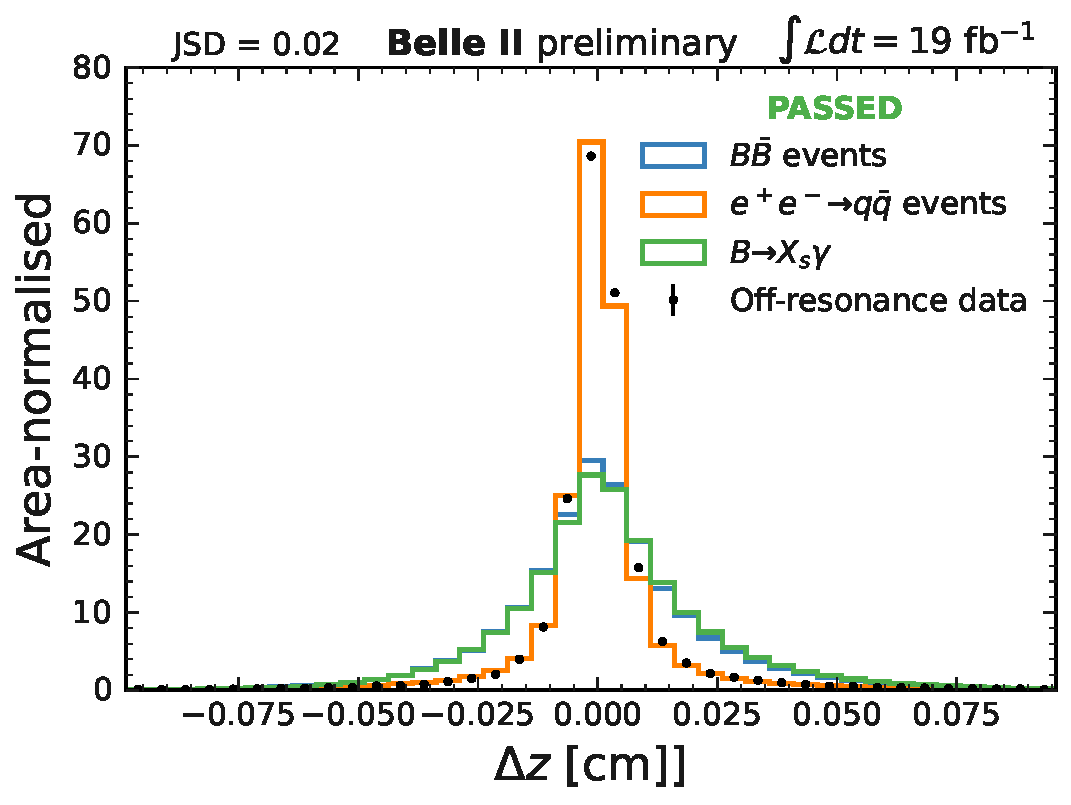
\includegraphics[width=0.3\textwidth]{figures/appendices/continuum_suppression_features/datamc_agreement_tests/Btag_DeltaZ_agreement_tested.pdf}    
    }
    \subcaptionbox{\label{fig:Btag_DeltaBoost_agreement_tested}}{
        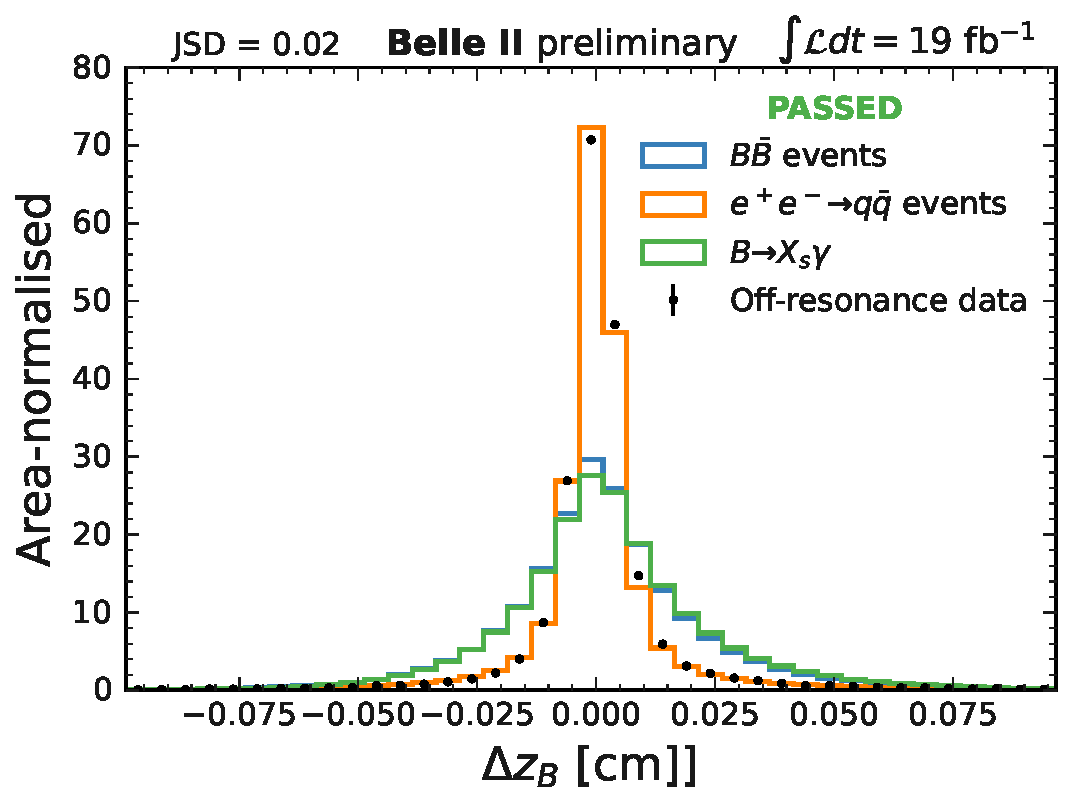
\includegraphics[width=0.3\textwidth]{figures/appendices/continuum_suppression_features/datamc_agreement_tests/Btag_DeltaBoost_agreement_tested.pdf}    
    }
    \subcaptionbox{\label{fig:Btag_TagVChi2IP_agreement_tested}}{
        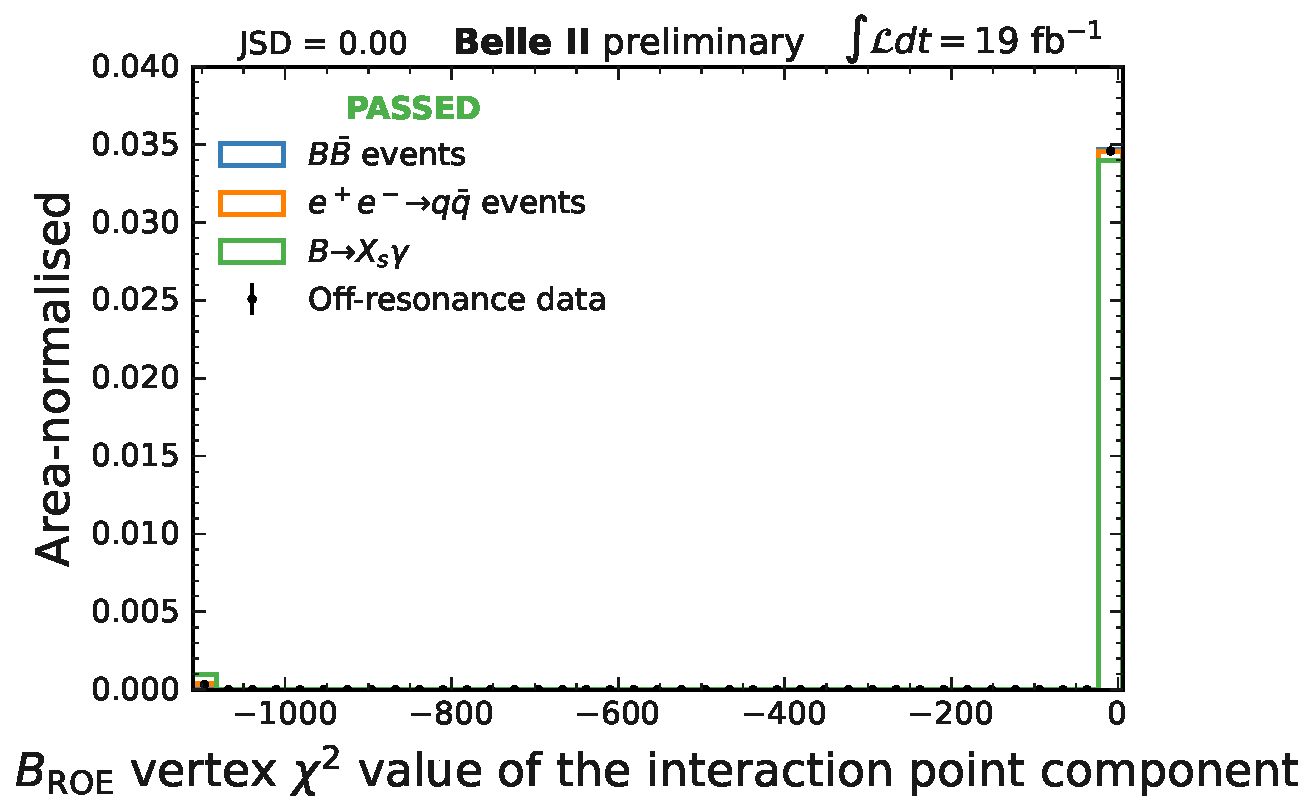
\includegraphics[width=0.3\textwidth]{figures/appendices/continuum_suppression_features/datamc_agreement_tests/Btag_TagVChi2IP_agreement_tested.pdf}    
    }
    \subcaptionbox{\label{fig:Btag_TagVxBeam_agreement_tested}}{
        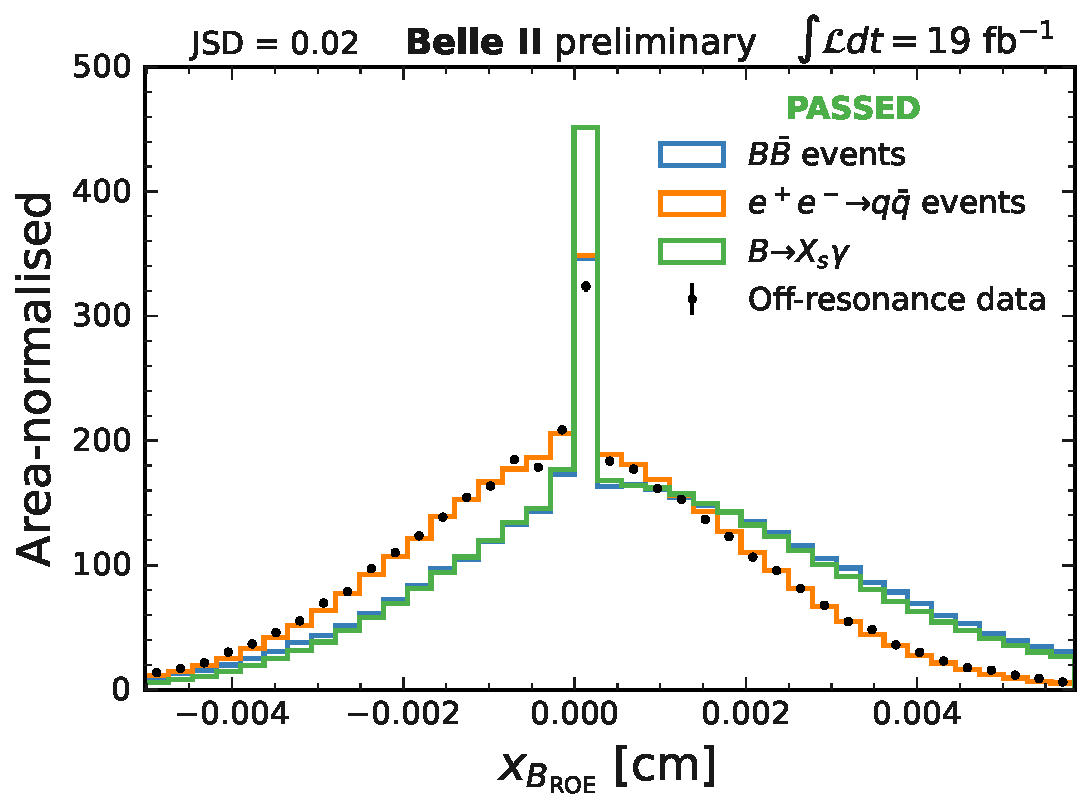
\includegraphics[width=0.3\textwidth]{figures/appendices/continuum_suppression_features/datamc_agreement_tests/Btag_TagVxBeam_agreement_tested.pdf}    
    }
    \subcaptionbox{\label{fig:Btag_TagVyBeam_agreement_tested}}{
        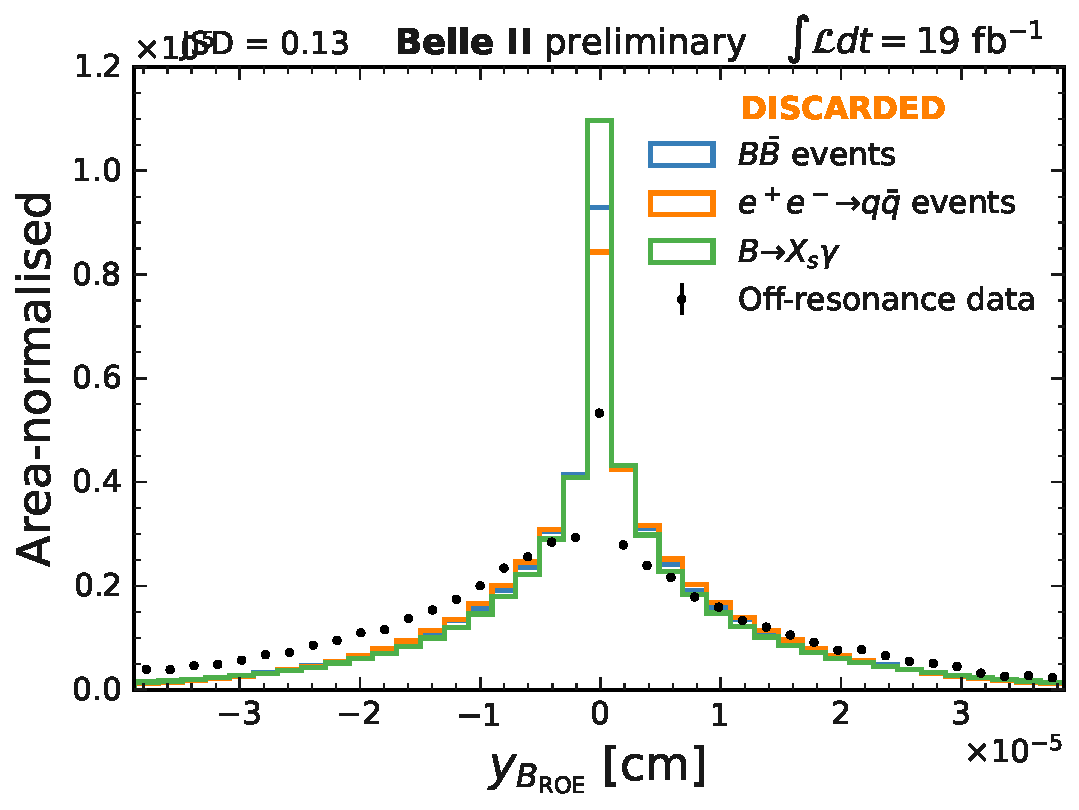
\includegraphics[width=0.3\textwidth]{figures/appendices/continuum_suppression_features/datamc_agreement_tests/Btag_TagVyBeam_agreement_tested.pdf}    
    }
    \subcaptionbox{\label{fig:Btag_TagVzBeam_agreement_tested}}{
        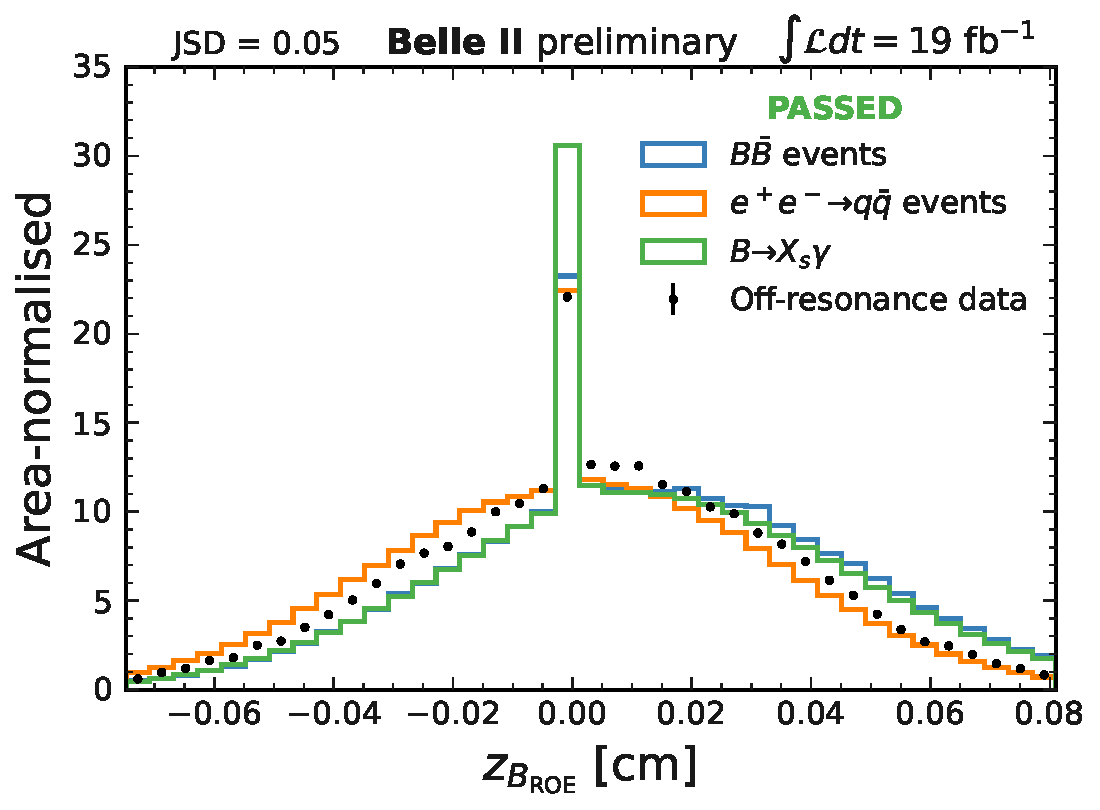
\includegraphics[width=0.3\textwidth]{figures/appendices/continuum_suppression_features/datamc_agreement_tests/Btag_TagVzBeam_agreement_tested.pdf}    
    }
    \caption{\label{fig:continuum_features_datamc_agreement} The data-simulation agreement test between \epem\ra\qqbar simulation and off-resonance Belle II data.
    The distributions shown are area-normalised, such that only a shape, but not a normalisation agreement test is performed.
    The Jensen-Shannon distance is evaluated between simulated \epem\ra\qqbar and off-resonance data distributions.
    For reference, also \BtoXsgamma and generic-\BB decay distributions are given.}
\end{figure}